\documentclass[aspectratio=169]{beamer}
\usetheme{Madrid}
\usecolortheme{default}

\usepackage[utf8]{inputenc}
\usepackage[T1]{fontenc}
\usepackage{amsmath}
\usepackage{amssymb}
\usepackage{graphicx}
\usepackage{tikz}
\usetikzlibrary{shapes.geometric,positioning,arrows.meta}
\usepackage{algorithm}
\usepackage{algpseudocode}

\title{LSE-PE: Log-Sum-Exp Processing Element}
\subtitle{Log-Sum-Exp Processing Element}
\author{Robin Warichet}
\date{}

\begin{document}

\frame{\titlepage}

\begin{frame}{Table des matières}
\tableofcontents
\end{frame}

\section{Contexte et Motivation}

\begin{frame}{Le Problème}
\begin{block}{Limites des DNNs}
\begin{itemize}
\item Manque d'interprétabilité
\item Sur-confiance dans les prédictions
\item Coût de calcul élevé
\end{itemize}
\end{block}

\begin{block}{Solution: Modèles Probabilistes (PMs)}
\begin{itemize}
\item Transparence et fiabilité
\item Estimation d'incertitude
\item Détection d'outliers
\end{itemize}
\end{block}

\vspace{0.3cm}
\textbf{Défi:} Calculer des probabilités très petites (ex: $2^{-12000}$)
\end{frame}

\begin{frame}{Pourquoi le Domaine Logarithmique?}
\begin{columns}
\column{0.5\textwidth}
\textbf{Domaine Linéaire}
\begin{itemize}
\item Multiplication: $a \times b$
\item Addition: $a + b$
\item \alert{Underflow} pour petites valeurs
\item FP32 limité: $2^{-126}$ à $2^{127}$
\end{itemize}

\column{0.5\textwidth}
\textbf{Domaine Logarithmique}
\begin{itemize}
\item Multiplication: $\log(a) + \log(b)$ ✓
\item Addition: $\log(a + b) = ?$ ✗
\item Pas d'underflow
\item Range étendu: $2^{-16384}$ à $2^0$
\end{itemize}
\end{columns}

\vspace{0.5cm}
\begin{alertblock}{Challenge Principal}
Comment calculer efficacement l'addition logarithmique?
\end{alertblock}
\end{frame}

\section{Circuits Probabilistes (PCs)}

\begin{frame}{Circuits Probabilistes: Structure}
\begin{columns}
\column{0.5\textwidth}
\begin{itemize}
\item Graphe acyclique dirigé (DAG)
\item Nœuds somme ($\oplus$) et produit ($\otimes$)
\item Feuilles: distributions simples
\item Calcul bottom-up
\end{itemize}

\vspace{0.3cm}
\textbf{Propriétés:}
\begin{itemize}
\item Inférence exacte
\item Temps polynomial
\item Expressivité élevée
\end{itemize}

\column{0.5\textwidth}
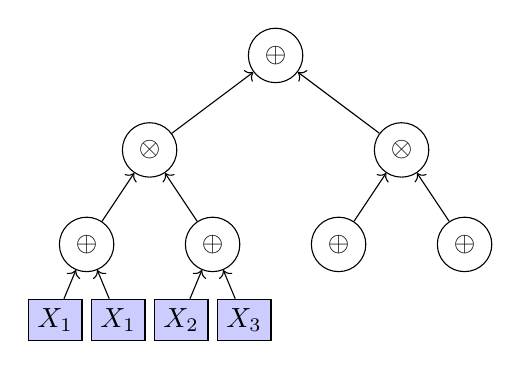
\begin{tikzpicture}[scale=0.8]
% Root
\node[circle,draw] (root) at (0,0) {$\oplus$};

% Second level
\node[circle,draw] (p1) at (-2,-1.5) {$\otimes$};
\node[circle,draw] (p2) at (2,-1.5) {$\otimes$};

% Third level
\node[circle,draw] (s1) at (-3,-3) {$\oplus$};
\node[circle,draw] (s2) at (-1,-3) {$\oplus$};
\node[circle,draw] (s3) at (1,-3) {$\oplus$};
\node[circle,draw] (s4) at (3,-3) {$\oplus$};

% Leaves
\node[rectangle,draw,fill=blue!20] (x1) at (-3.5,-4.2) {$X_1$};
\node[rectangle,draw,fill=blue!20] (x2) at (-2.5,-4.2) {$X_1$};
\node[rectangle,draw,fill=blue!20] (x3) at (-1.5,-4.2) {$X_2$};
\node[rectangle,draw,fill=blue!20] (x4) at (-0.5,-4.2) {$X_3$};

% Connections
\draw[->] (p1) -- (root);
\draw[->] (p2) -- (root);
\draw[->] (s1) -- (p1);
\draw[->] (s2) -- (p1);
\draw[->] (s3) -- (p2);
\draw[->] (s4) -- (p2);
\draw[->] (x1) -- (s1);
\draw[->] (x2) -- (s1);
\draw[->] (x3) -- (s2);
\draw[->] (x4) -- (s2);
\end{tikzpicture}
\end{columns}
\end{frame}

\begin{frame}{Cas d'Usage: Détection d'Outliers}
\begin{center}
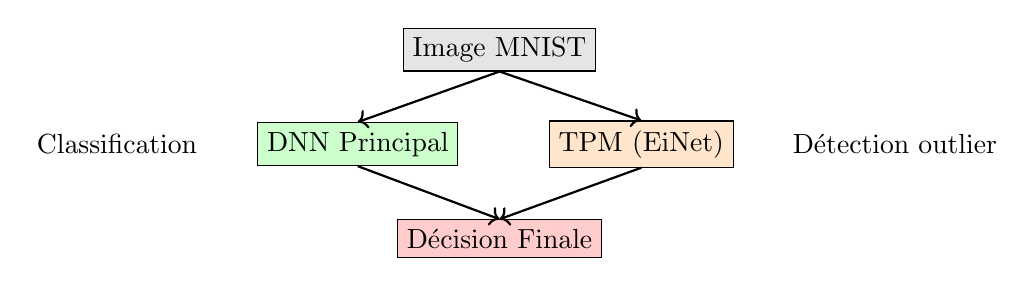
\begin{tikzpicture}[scale=1.2]
% Input
\node[rectangle,draw,fill=gray!20] (input) at (0,0) {Image MNIST};

% DNN
\node[rectangle,draw,fill=green!20] (dnn) at (-1.5,-1) {DNN Principal};
\node[right] at (-5,-1) {Classification};

% TPM
\node[rectangle,draw,fill=orange!20] (tpm) at (1.5,-1) {TPM (EiNet)};
\node[right] at (3,-1) {Détection outlier};

% Output
\node[rectangle,draw,fill=red!20] (decision) at (0,-2) {Décision Finale};

% Arrows with proper anchors
\draw[->,thick] (input.south) -- (dnn.north);
\draw[->,thick] (input.south) -- (tpm.north);
\draw[->,thick] (dnn.south) -- (decision.north);
\draw[->,thick] (tpm.south) -- (decision.north);
\end{tikzpicture}
\end{center}

\vspace{0.3cm}
\textbf{Avantages:}
\begin{itemize}
\item TPM léger: 20k MACs vs 416k-18M MACs pour le DNN
\item Détecte les données hors distribution
\item Coût: 0.4\% à 20\% du modèle principal
\end{itemize}
\end{frame}

\section{Fonction Log-Sum-Exp (LSE)}

\begin{frame}{La Fonction LSE}
\begin{block}{Définition}
Pour éviter l'underflow en domaine log:
\[
\text{LSE}(x, y) = c + \log\left(e^{x-c} + e^{y-c}\right)
\]
où $c = \max(x, y)$
\end{block}

\begin{block}{Simplification (avec $x \geq y$)}
\[
\text{LSE}(x, y) = x + \log\left(1 + e^{y-x}\right) = x + f(y-x)
\]
\end{block}

\vspace{0.3cm}
\textbf{Problème:} Calcul de $f(y-x) = \log(1 + 2^{y-x})$ coûteux en hardware
\begin{itemize}
\item Opérations exponentielles et logarithmiques
\item LUTs de taille exponentielle
\item Ressources importantes
\end{itemize}
\end{frame}

\begin{frame}{État de l'Art: Limitations}
\begin{table}
\small
\begin{tabular}{|l|c|c|c|}
\hline
\textbf{Méthode} & \textbf{Range} & \textbf{Erreur} & \textbf{Coût} \\
\hline
FP32 & $2^{-126}$ à $2^{127}$ & Haute & Faible \\
\hline
Posit32 & $2^{-120}$ à $2^{120}$ & Haute & Faible \\
\hline
Custom Posit32 & $2^{-1920}$ à $2^{1920}$ & Moyenne & Moyen \\
\hline
Order-2 LUT & $2^{-512}$ à $2^{0}$ & $2^{-19.5}$ & \alert{Très élevé} \\
\hline
No LUT & $2^{-64}$ à $2^{63}$ & \alert{$3.4 \times 10^{17}$} & Faible \\
\hline
\textbf{LSE-PE (proposé)} & \textbf{$2^{-16384}$ à $2^{0}$} & \textbf{0.001} & \textbf{Faible} \\
\hline
\end{tabular}
\end{table}

\vspace{0.5cm}
\begin{alertblock}{Besoin}
Un système avec large range, haute précision ET faible coût matériel
\end{alertblock}
\end{frame}

\section{Architecture LSE-PE}

\begin{frame}{Principe: Double Approximation}
\textbf{Objectif:} Approximer $f(y-x) = \log_2(1 + 2^{y-x})$

\vspace{0.3cm}
\begin{block}{Étape 1: Approximation Exponentielle (gexp)}
\[
2^z \approx z + 1 \quad \text{(Approximation de Mitchell)}
\]
Donc: $2^{y-x} = 2^{I_{y-x}} \cdot 2^{F_{y-x}} \approx (1 + F_{y-x}) \gg (-I_{y-x})$
\end{block}

\begin{block}{Étape 2: Approximation Logarithmique ($f_{\log}$)}
\[
\log_2(1 + z) \approx z
\]
Donc: $\log_2(1 + 2^{y-x}) \approx (1 + F_{y-x}) \gg (-I_{y-x})$
\end{block}

\vspace{0.3cm}
\textbf{Résultat:} $\tilde{f}(y-x) = (1 + F_{y-x}) \gg (-I_{y-x})$ \\
$\rightarrow$ Seulement des additions et bit-shifts!
\end{frame}

\begin{frame}{Correction d'Erreur avec CLUT}
\begin{columns}
\column{0.5\textwidth}
\textbf{Problème:}
\begin{itemize}
\item Approximation introduit erreur max 0.085
\item $\tilde{f}(y-x) \in [0, 1)$ toujours
\end{itemize}

\vspace{0.3cm}
\textbf{Solution: CLUT}
\begin{itemize}
\item Correction LUT compacte
\item 16 entrées × 10 bits
\item Interpolation linéaire
\item Range fixe [0, 1)
\end{itemize}

\column{0.5\textwidth}
\begin{figure}
    \centering
    \includegraphics[width=\linewidth]{présentation 1/Capture d’écran 2025-10-05 185036.png}
    \caption{Error of $\tilde{f}_{(y−x)}$ under different approximations}
   \label{fig:tilde-error}
\end{figure}
\end{columns}

\begin{block}{Formule Finale}
\[
\text{LSE-PE}(x, y) \approx x + \tilde{f}(y-x) + \text{CLUT}(\tilde{f}(y-x))
\]
\end{block}
\end{frame}

\begin{frame}[fragile]{Algorithme LSE-PE}
\begin{algorithmic}[1]
\Function{LSE-PE}{$x, y$}
\State Supposer $x \geq y$
\State $\text{Sub} \gets y - x$
\State $I_{(y-x)} \gets \text{Int}(\text{Sub})$, $F_{(y-x)} \gets \text{Frac}(\text{Sub})$
\State
\State \textcolor{blue}{// Approximation double}
\State $\tilde{f}(y-x) \gets (1 + F_{(y-x)}) \gg (-I_{(y-x)})$
\State
\State \textcolor{blue}{// Correction d'erreur}
\State \Return $x + \tilde{f}(y-x) + \text{CLUT}(\tilde{f}(y-x))$
\EndFunction
\end{algorithmic}

\vspace{0.5cm}
\textbf{Complexité:} 
\begin{itemize}
\item 1 comparaison, 1 soustraction, 2 additions, 1 bit-shift
\item 1 accès CLUT (16 entrées seulement)
\end{itemize}
\end{frame}

\begin{frame}{Implémentation Matérielle}

\begin{figure}
    \centering
    \includegraphics[width=0.5\linewidth]{présentation 1/Capture d'écran 2025-10-05 184317.png}
    \caption{Implementation of 64 parallel MAC units using
LSE-PE as logarithmic adders (LSE-PE), fixed-point adder as
logarithmic multipliers (MULT.).}
   \label{fig:lse-mac-implementation}
\end{figure}
    
\end{frame}

\begin{frame}{Résultats de Validation}
\begin{table}
\small
\begin{tabular}{|l|c|c|c|}
\hline
\textbf{Module} & \textbf{Tests} & \textbf{Succès} & \textbf{Taux} \\
\hline
LSE Add & 40 & 47 & \textcolor{yellow}{\textbf{85.1\%}} \\
\hline
LSE Mult & 14 & 14 & \textcolor{green}{\textbf{100\%}} \\
\hline
\end{tabular}
\end{table}

\vspace{0.3cm}
\textbf{Tests Système Validés:}
\begin{itemize}
\item  Opération MAC simple
\item  Opérations MAC parallèles (4 unités)
\item  Opérations MAC séquentielles
\item  Mode bypass
\item  Test de stress multi-itérations
\end{itemize}
\end{frame}

\begin{frame}{Optimisations possible}
\begin{enumerate}
\item \textbf{CLUT Partagée} (vs CLUT individuelle)
   \begin{itemize}
   \item de réduction de surface
   \item Pas de perte de performance grâce au pipeline
   \end{itemize}

\item \textbf{Double Mode Opératoire}
   \begin{itemize}
   \item 24-bit: haute précision pour modèles complexes
   \item SIMD 4×6-bit: 4× débit pour réseaux compacts
   \end{itemize}

\item \textbf{Pipeline Optimisé}
   \begin{itemize}
   \item Latence fixe: 3 cycles
   \item Interface ready/valid pour backpressure
   \item Gestion accumulator avec first\_op\_after\_load
   \end{itemize}

\item \textbf{Infrastructure de Test Complète}
   \begin{itemize}
   \item Testbenches SystemVerilog automatisés
   \item Scripts PowerShell pour validation continue
   \end{itemize}
\end{enumerate}
\end{frame}

\begin{frame}{Bloc LSE Mult SIMD}
\begin{columns}
\column{0.52\textwidth}
\begin{itemize}
   \item Architecture hiérarchique: \textit{lanes} 1\,×\,24, 2\,×\,12 ou 4\,×\,6 bits
   \item \textbf{Full adders} chaînés pour chaque lane avec remise à zéro du carry
   \item \textbf{Mux} paramétriques contrôlés par \texttt{mode} pour isoler les lanes
   \item Entrées synchronisées via pipeline léger (mode combinatoire possible)
   \item Interface simple: \texttt{a}, \texttt{b}, \texttt{mode} $\rightarrow$ \texttt{sum}, \texttt{carry	extunderscore out}
\end{itemize}

\column{0.48\textwidth}
\begin{tikzpicture}[x=1.1cm,y=0.9cm,>=Latex,thick]
   	ikzset{
      signal/.style={draw,fill=blue!10,minimum width=2.2cm,minimum height=0.9cm},
      mux/.style={draw,fill=orange!25,trapezium,trapezium left angle=70,trapezium right angle=110,minimum width=1.8cm,minimum height=1.0cm},
      splitter/.style={draw,fill=green!15,minimum width=2.4cm,minimum height=0.9cm,rounded corners=2pt},
      adder/.style={draw,fill=purple!15,minimum width=2.0cm,minimum height=0.9cm,rounded corners=2pt},
      reg/.style={draw,fill=cyan!15,minimum width=1.4cm,minimum height=0.9cm},
      bus/.style={line width=1pt}
   }

   % Inputs
   \node[signal] (inA) at (0,2.2) {$A[23:0]$};
   \node[signal] (inB) at (0,1.0) {$B[23:0]$};
   \node[reg] (modeReg) at (0,-0.3) {mode};

   % Draw clock triangle for register
   \draw (modeReg.west)+(0,0.15) -- ++(-0.35,-0.15) -- ++(0.35,-0.15) -- cycle;

   \node[mux,anchor=west] (muxMask) at (1.8,1.6) {Mux masque};
   \node[splitter,anchor=west] (lanes) at (3.3,1.6) {Gating lanes};

   % Lane full adder chains
   \node[adder,anchor=west] (fa0) at (5.2,2.4) {Lane 0: FA $\times 6$};
   \node[adder,anchor=west] (fa1) at (5.2,1.6) {Lane 1: FA $\times 6$};
   \node[adder,anchor=west] (fa2) at (5.2,0.8) {Lane 2: FA $\times 6$};
   \node[adder,anchor=west] (fa3) at (5.2,0.0) {Lane 3: FA $\times 6$};

   % Output register and carry mux
   \node[reg,anchor=west] (sumReg) at (7.4,1.6) {sum};
   \draw (sumReg.west)+(0,0.15) -- ++(-0.35,-0.15) -- ++(0.35,-0.15) -- cycle;
   \node[mux,anchor=west] (carryMux) at (7.4,0.1) {Mux carry};
   \node[signal,anchor=west] (sumOut) at (9.0,1.6) {Sortie $sum[23:0]$};
   \node[signal,anchor=west] (carryOut) at (9.0,0.1) {$carry\_{lane}$};

   % Connections
   \draw[->,bus] (inA.east) -- ++(0.4,0) |- (muxMask.140);
   \draw[->,bus] (inB.east) -- ++(0.4,0) |- (muxMask.220);
   \draw[->] (modeReg.east) -- ++(0.4,0) |- (muxMask.270);

   \draw[->,bus] (muxMask.east) -- (lanes.west);
   \coordinate (split) at ($(lanes.east)+(0.5,0)$);
   \draw[->,bus] (lanes.east) -- (split);

   % Split connections to adders
   \foreach \offset/\target in {0.9/fa0.west,0.3/fa1.west,-0.3/fa2.west,-0.9/fa3.west}{%
      \draw[->,bus] (split) |- ($(split)+(0,\offset)$) -- (\target);
   }

   % Outputs from adders
   \draw[->,bus] (fa0.east) -- ++(0.5,0) |- (sumReg.west);
   \draw[->,bus] (fa1.east) -- ++(0.5,0) |- (sumReg.west);
   \draw[->,bus] (fa2.east) -- ++(0.5,0) |- (sumReg.west);
   \draw[->,bus] (fa3.east) -- ++(0.5,0) |- (sumReg.west);
   \draw[->,bus] (fa3.east) -- ++(0.5,-0.8) |- (carryMux.west);

   \draw[->,bus] (sumReg.east) -- (sumOut.west);
   \draw[->] (carryMux.east) -- (carryOut.west);
\end{tikzpicture}
\label{fig:lse-mult-simd-architecture}
\end{columns}
\end{frame}

\section{Conclusion}

\begin{frame}{Conclusion}
\begin{center}
\Huge Merci pour votre attention!

\vspace{1cm}
\large
\textbf{LSE-PE: Hardware Efficace pour\\Raisonnement Probabiliste Tractable}

\vspace{0.5cm}
\normalsize
Robin Warichet

\vspace{1cm}
\end{center}
\end{frame}

\end{document}